\documentclass[tikz,border=2pt]{standalone}
% Shared look for the paper's diagrams (built standalone: figures/diagrams/Makefile).
\usepackage[T1]{fontenc}
\usepackage{newtxtext,newtxmath}
\usepackage{xcolor}
\usepackage{tikz}
\usetikzlibrary{positioning,arrows.meta,fit,calc,backgrounds,decorations.pathreplacing}
\definecolor{ink}{HTML}{1F2328}
\definecolor{muted}{HTML}{6A737D}
\definecolor{rulec}{HTML}{D0D4DC}
\definecolor{fillc}{HTML}{F4F5F8}
\definecolor{sone}{HTML}{2A78D6}   % categorical slot 1: Kubernetes Job / trees
\definecolor{stwo}{HTML}{EB6834}   % slot 2: language models
\definecolor{sthree}{HTML}{1BAF7A} % slot 3: combinations
\definecolor{flyte}{HTML}{6250D6}
\tikzset{
  >={Stealth[length=5pt,width=4pt]},
  every node/.style={font=\small, text=ink},
  box/.style={draw=rulec, fill=white, rounded corners=2pt, inner sep=5pt, line width=0.6pt, align=left},
  head/.style={font=\scriptsize\bfseries\sffamily, text=muted},
  note/.style={font=\scriptsize, text=muted, align=left},
  flow/.style={->, draw=muted, line width=0.7pt},
}

\begin{document}
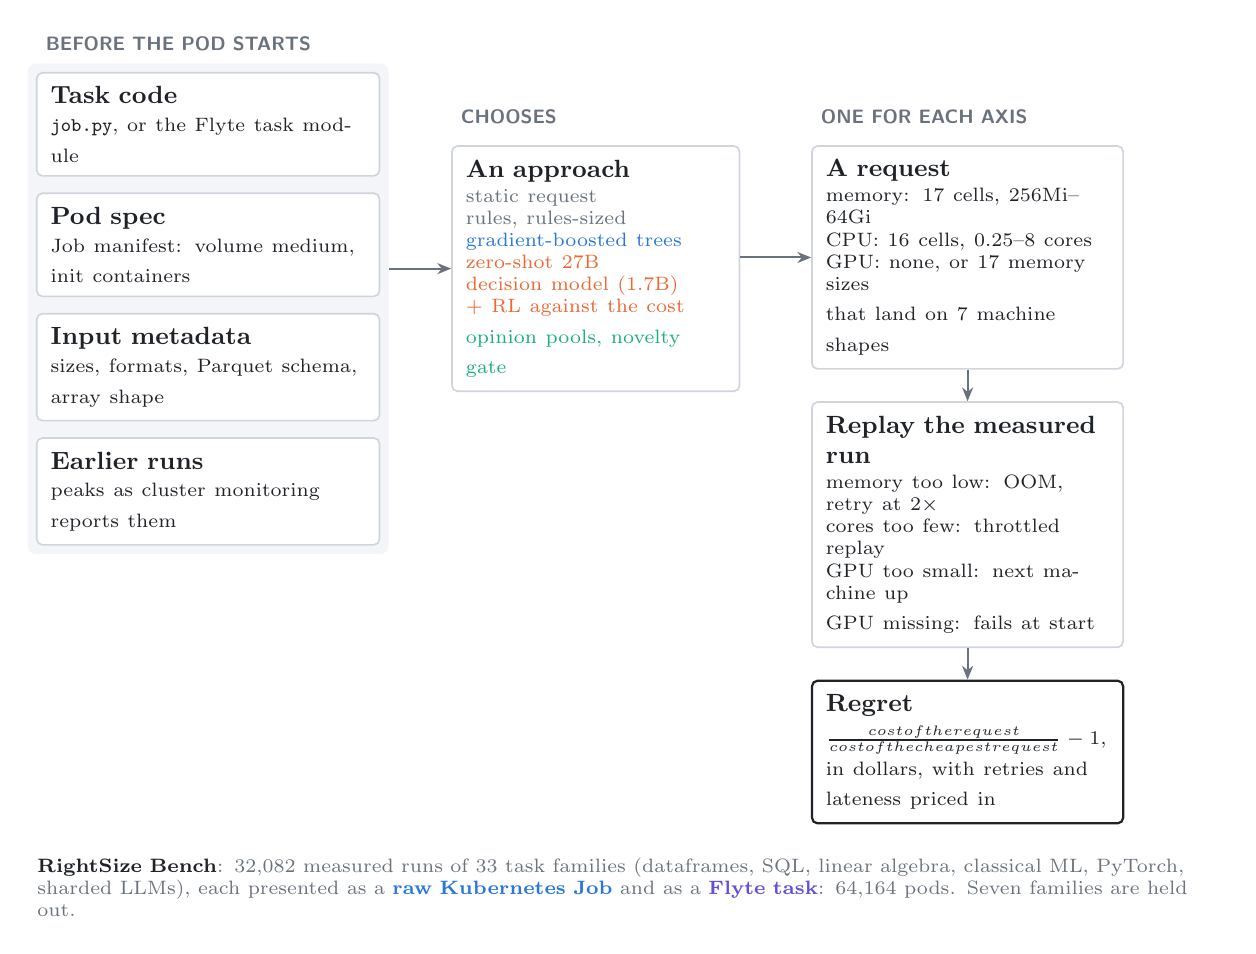
\begin{tikzpicture}[node distance=4mm]
% what a scheduler can read
\node[head] (h1) {BEFORE THE POD STARTS};
\node[box, below=1.5mm of h1.south west, anchor=north west, text width=40mm] (code) {\textbf{Task code}\\[-1pt]{\scriptsize\texttt{job.py}, or the Flyte task module}};
\node[box, below=2mm of code, text width=40mm] (spec) {\textbf{Pod spec}\\[-1pt]{\scriptsize Job manifest: volume medium, init containers}};
\node[box, below=2mm of spec, text width=40mm] (inp) {\textbf{Input metadata}\\[-1pt]{\scriptsize sizes, formats, Parquet schema, array shape}};
\node[box, below=2mm of inp, text width=40mm] (hist) {\textbf{Earlier runs}\\[-1pt]{\scriptsize peaks as cluster monitoring reports them}};

% approaches
\node[box, right=9mm of spec.north east, anchor=north west, text width=33mm, yshift=6mm] (appr) {%
\textbf{An approach}\\[1pt]
{\scriptsize\color{muted}static request\\ rules, rules-sized\\}
{\scriptsize\color{sone}gradient-boosted trees\\}
{\scriptsize\color{stwo}zero-shot 27B\\ decision model (1.7B)\\ + RL against the cost\\}
{\scriptsize\color{sthree}opinion pools, novelty gate}};
\node[head, above=1.5mm of appr.north west, anchor=south west] {CHOOSES};

% request
\node[box, right=9mm of appr.north east, anchor=north west, text width=36mm] (req) {%
\textbf{A request}\\[1pt]
{\scriptsize memory: 17 cells, 256Mi--64Gi\\ CPU: 16 cells, 0.25--8 cores\\ GPU: none, or 17 memory sizes\\ that land on 7 machine shapes}};
\node[head, above=1.5mm of req.north west, anchor=south west] {ONE FOR EACH AXIS};

% simulator
\node[box, below=4mm of req, text width=36mm] (sim) {%
\textbf{Replay the measured run}\\[1pt]
{\scriptsize memory too low: OOM, retry at 2$\times$\\ cores too few: throttled replay\\ GPU too small: next machine up\\ GPU missing: fails at start}};

\node[box, below=4mm of sim, text width=36mm, draw=ink, line width=0.8pt] (reg) {%
\textbf{Regret}\\[1pt]
{\scriptsize $\frac{\text{cost of the request}}{\text{cost of the cheapest request}} - 1$, in dollars, with retries and lateness priced in}};

\begin{scope}[on background layer]
\node[fit=(code)(hist), draw=none, fill=fillc, rounded corners=3pt, inner sep=3pt] (readbg) {};
\end{scope}
\draw[flow] (readbg.east |- appr.west) -- (appr.west);
\draw[flow] (appr.east |- req.west) -- (req.west);
\draw[flow] (req) -- (sim);
\draw[flow] (sim) -- (reg);

% the benchmark underneath
\node[note, anchor=north west, text width=150mm] (bench) at ([yshift=-3mm]current bounding box.south west) {%
{\color{ink}\textbf{RightSize Bench}}: 32,082 measured runs of 33 task families (dataframes, SQL, linear algebra,
classical ML, PyTorch, sharded LLMs), each presented as a {\color{sone}\textbf{raw Kubernetes Job}} and as a
{\color{flyte}\textbf{Flyte task}}: 64,164 pods. Seven families are held out.};
\end{tikzpicture}
\end{document}
